\documentclass[twoside]{book}

% Packages required by doxygen
\usepackage{fixltx2e}
\usepackage{calc}
\usepackage{doxygen}
\usepackage[export]{adjustbox} % also loads graphicx
\usepackage{graphicx}
\usepackage[utf8]{inputenc}
\usepackage{makeidx}
\usepackage{multicol}
\usepackage{multirow}
\PassOptionsToPackage{warn}{textcomp}
\usepackage{textcomp}
\usepackage[nointegrals]{wasysym}
\usepackage[table]{xcolor}

% Font selection
\usepackage[T1]{fontenc}
\usepackage[scaled=.90]{helvet}
\usepackage{courier}
\usepackage{amssymb}
\usepackage{sectsty}
\renewcommand{\familydefault}{\sfdefault}
\allsectionsfont{%
  \fontseries{bc}\selectfont%
  \color{darkgray}%
}
\renewcommand{\DoxyLabelFont}{%
  \fontseries{bc}\selectfont%
  \color{darkgray}%
}
\newcommand{\+}{\discretionary{\mbox{\scriptsize$\hookleftarrow$}}{}{}}

% Page & text layout
\usepackage{geometry}
\geometry{%
  a4paper,%
  top=2.5cm,%
  bottom=2.5cm,%
  left=2.5cm,%
  right=2.5cm%
}
\tolerance=750
\hfuzz=15pt
\hbadness=750
\setlength{\emergencystretch}{15pt}
\setlength{\parindent}{0cm}
\setlength{\parskip}{3ex plus 2ex minus 2ex}
\makeatletter
\renewcommand{\paragraph}{%
  \@startsection{paragraph}{4}{0ex}{-1.0ex}{1.0ex}{%
    \normalfont\normalsize\bfseries\SS@parafont%
  }%
}
\renewcommand{\subparagraph}{%
  \@startsection{subparagraph}{5}{0ex}{-1.0ex}{1.0ex}{%
    \normalfont\normalsize\bfseries\SS@subparafont%
  }%
}
\makeatother

% Headers & footers
\usepackage{fancyhdr}
\pagestyle{fancyplain}
\fancyhead[LE]{\fancyplain{}{\bfseries\thepage}}
\fancyhead[CE]{\fancyplain{}{}}
\fancyhead[RE]{\fancyplain{}{\bfseries\leftmark}}
\fancyhead[LO]{\fancyplain{}{\bfseries\rightmark}}
\fancyhead[CO]{\fancyplain{}{}}
\fancyhead[RO]{\fancyplain{}{\bfseries\thepage}}
\fancyfoot[LE]{\fancyplain{}{}}
\fancyfoot[CE]{\fancyplain{}{}}
\fancyfoot[RE]{\fancyplain{}{\bfseries\scriptsize Generated by Doxygen }}
\fancyfoot[LO]{\fancyplain{}{\bfseries\scriptsize Generated by Doxygen }}
\fancyfoot[CO]{\fancyplain{}{}}
\fancyfoot[RO]{\fancyplain{}{}}
\renewcommand{\footrulewidth}{0.4pt}
\renewcommand{\chaptermark}[1]{%
  \markboth{#1}{}%
}
\renewcommand{\sectionmark}[1]{%
  \markright{\thesection\ #1}%
}

% Indices & bibliography
\usepackage{natbib}
\usepackage[titles]{tocloft}
\setcounter{tocdepth}{3}
\setcounter{secnumdepth}{5}
\makeindex

% Hyperlinks (required, but should be loaded last)
\usepackage{ifpdf}
\ifpdf
  \usepackage[pdftex,pagebackref=true]{hyperref}
\else
  \usepackage[ps2pdf,pagebackref=true]{hyperref}
\fi
\hypersetup{%
  colorlinks=true,%
  linkcolor=blue,%
  citecolor=blue,%
  unicode%
}

% Custom commands
\newcommand{\clearemptydoublepage}{%
  \newpage{\pagestyle{empty}\cleardoublepage}%
}

\usepackage{caption}
\captionsetup{labelsep=space,justification=centering,font={bf},singlelinecheck=off,skip=4pt,position=top}

%===== C O N T E N T S =====

\begin{document}

% Titlepage & ToC
\hypersetup{pageanchor=false,
             bookmarksnumbered=true,
             pdfencoding=unicode
            }
\pagenumbering{alph}
\begin{titlepage}
\vspace*{7cm}
\begin{center}%
{\Large Documentation \\[1ex]\large 1 }\\
\vspace*{1cm}
{\large Generated by Doxygen 1.8.13}\\
\end{center}
\end{titlepage}
\clearemptydoublepage
\pagenumbering{roman}
\tableofcontents
\clearemptydoublepage
\pagenumbering{arabic}
\hypersetup{pageanchor=true}

%--- Begin generated contents ---
\chapter{Hierarchical Index}
\section{Class Hierarchy}
This inheritance list is sorted roughly, but not completely, alphabetically\+:\begin{DoxyCompactList}
\item \contentsline{section}{gamestate}{\pageref{classgamestate}}{}
\item Q\+Graphics\+Pixmap\+Item\begin{DoxyCompactList}
\item \contentsline{section}{arrow}{\pageref{classarrow}}{}
\item \contentsline{section}{bow}{\pageref{classbow}}{}
\item \contentsline{section}{myplayer1}{\pageref{classmyplayer1}}{}
\item \contentsline{section}{scoreboard}{\pageref{classscoreboard}}{}
\item \contentsline{section}{target}{\pageref{classtarget}}{}
\end{DoxyCompactList}
\item Q\+Graphics\+Text\+Item\begin{DoxyCompactList}
\item \contentsline{section}{score}{\pageref{classscore}}{}
\end{DoxyCompactList}
\item Q\+Object\begin{DoxyCompactList}
\item \contentsline{section}{arrow}{\pageref{classarrow}}{}
\item \contentsline{section}{client}{\pageref{classclient}}{}
\item \contentsline{section}{screen\+Update}{\pageref{classscreen_update}}{}
\item \contentsline{section}{server}{\pageref{classserver}}{}
\item \contentsline{section}{target}{\pageref{classtarget}}{}
\end{DoxyCompactList}
\end{DoxyCompactList}

\chapter{Class Index}
\section{Class List}
Here are the classes, structs, unions and interfaces with brief descriptions\+:\begin{DoxyCompactList}
\item\contentsline{section}{\hyperlink{classarrow}{arrow} \\*The Class to Create an Arrow Object }{\pageref{classarrow}}{}
\item\contentsline{section}{\hyperlink{classbow}{bow} \\*The Class to create Bow object }{\pageref{classbow}}{}
\item\contentsline{section}{\hyperlink{classclient}{client} \\*Classs to Create Client }{\pageref{classclient}}{}
\item\contentsline{section}{\hyperlink{classgamestate}{gamestate} \\*Class to store the State of the Game }{\pageref{classgamestate}}{}
\item\contentsline{section}{\hyperlink{classmyplayer1}{myplayer1} \\*Class to create Player Object }{\pageref{classmyplayer1}}{}
\item\contentsline{section}{\hyperlink{classscore}{score} \\*Class to create Score Object }{\pageref{classscore}}{}
\item\contentsline{section}{\hyperlink{classscoreboard}{scoreboard} \\*Class to create Scoreboard Object }{\pageref{classscoreboard}}{}
\item\contentsline{section}{\hyperlink{classscreen_update}{screen\+Update} \\*Class to create Screen Updator Object }{\pageref{classscreen_update}}{}
\item\contentsline{section}{\hyperlink{classserver}{server} \\*Class to create Server }{\pageref{classserver}}{}
\item\contentsline{section}{\hyperlink{classtarget}{target} \\*Class to create Target object }{\pageref{classtarget}}{}
\end{DoxyCompactList}

\chapter{Class Documentation}
\hypertarget{classarrow}{}\section{arrow Class Reference}
\label{classarrow}\index{arrow@{arrow}}


The Class to Create an Arrow Object.  




{\ttfamily \#include $<$arrow.\+h$>$}

Inheritance diagram for arrow\+:\begin{figure}[H]
\begin{center}
\leavevmode
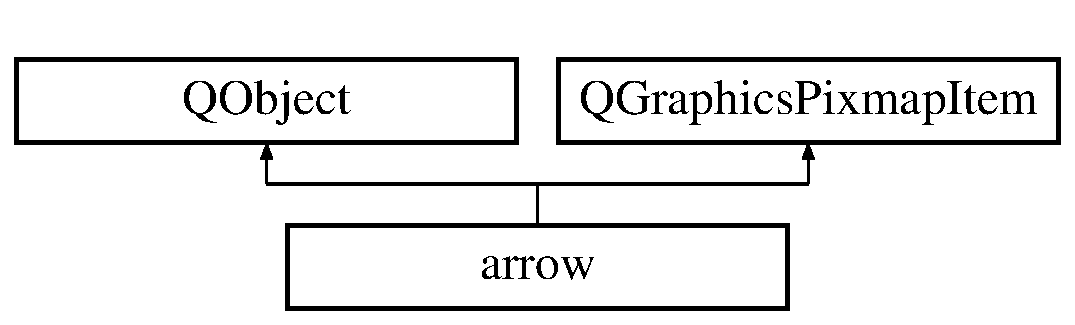
\includegraphics[height=2.000000cm]{classarrow}
\end{center}
\end{figure}
\subsection*{Public Slots}
\begin{DoxyCompactItemize}
\item 
\mbox{\Hypertarget{classarrow_aeffacc576310b21b006ddf225159f576}\label{classarrow_aeffacc576310b21b006ddf225159f576}} 
void \hyperlink{classarrow_aeffacc576310b21b006ddf225159f576}{move} ()
\begin{DoxyCompactList}\small\item\em Moves the arrow after it is launched. \end{DoxyCompactList}\end{DoxyCompactItemize}
\subsection*{Public Member Functions}
\begin{DoxyCompactItemize}
\item 
\hyperlink{classarrow_aad351384362146630ada6411bde30640}{arrow} (\hyperlink{classgamestate}{gamestate} $\ast$state\+\_\+param, \hyperlink{classtarget}{target} $\ast$t\+\_\+param)
\begin{DoxyCompactList}\small\item\em Arrow Constructor to create arrow for player1. \end{DoxyCompactList}\item 
\mbox{\Hypertarget{classarrow_a1d7f5d14c75ee5dccfdf8aee90e873dc}\label{classarrow_a1d7f5d14c75ee5dccfdf8aee90e873dc}} 
\hyperlink{classarrow_a1d7f5d14c75ee5dccfdf8aee90e873dc}{arrow} (int i)
\begin{DoxyCompactList}\small\item\em Arrow Constructor to create arrow for player2. \end{DoxyCompactList}\end{DoxyCompactItemize}
\subsection*{Public Attributes}
\begin{DoxyCompactItemize}
\item 
\mbox{\Hypertarget{classarrow_afbf525f81eb33ed7dca870bae3dc7adf}\label{classarrow_afbf525f81eb33ed7dca870bae3dc7adf}} 
\hyperlink{classgamestate}{gamestate} $\ast$ \hyperlink{classarrow_afbf525f81eb33ed7dca870bae3dc7adf}{state}
\begin{DoxyCompactList}\small\item\em Reference to the state of the game. \end{DoxyCompactList}\item 
\mbox{\Hypertarget{classarrow_a060b31937403d1059a127e579ff8f0d0}\label{classarrow_a060b31937403d1059a127e579ff8f0d0}} 
\hyperlink{classtarget}{target} $\ast$ \hyperlink{classarrow_a060b31937403d1059a127e579ff8f0d0}{t}
\begin{DoxyCompactList}\small\item\em Reference to the target in the game. \end{DoxyCompactList}\item 
\mbox{\Hypertarget{classarrow_aa84c13c4959f9481a6101a79067e9899}\label{classarrow_aa84c13c4959f9481a6101a79067e9899}} 
qreal \hyperlink{classarrow_aa84c13c4959f9481a6101a79067e9899}{angle}
\begin{DoxyCompactList}\small\item\em Angle at which the arrow was launched. \end{DoxyCompactList}\item 
\mbox{\Hypertarget{classarrow_a923436fb052435dc61bdefa72cef8a62}\label{classarrow_a923436fb052435dc61bdefa72cef8a62}} 
qreal \hyperlink{classarrow_a923436fb052435dc61bdefa72cef8a62}{present\+Angle}
\begin{DoxyCompactList}\small\item\em Stores the current angle of the arrow. \end{DoxyCompactList}\item 
\mbox{\Hypertarget{classarrow_adc3a32bcf6bf8c9d4ec8abe5398cfc4e}\label{classarrow_adc3a32bcf6bf8c9d4ec8abe5398cfc4e}} 
qreal \hyperlink{classarrow_adc3a32bcf6bf8c9d4ec8abe5398cfc4e}{initialX}
\begin{DoxyCompactList}\small\item\em X coordinate from where the arrow the was launched. \end{DoxyCompactList}\item 
\mbox{\Hypertarget{classarrow_a6f052d5f3dfce79d72564bac1a760e88}\label{classarrow_a6f052d5f3dfce79d72564bac1a760e88}} 
qreal \hyperlink{classarrow_a6f052d5f3dfce79d72564bac1a760e88}{initialY}
\begin{DoxyCompactList}\small\item\em Y coordinate from where the arrow the was launched. \end{DoxyCompactList}\item 
\mbox{\Hypertarget{classarrow_aba775d30acf4655d9ffeabcf998b69f5}\label{classarrow_aba775d30acf4655d9ffeabcf998b69f5}} 
qreal \hyperlink{classarrow_aba775d30acf4655d9ffeabcf998b69f5}{time}
\begin{DoxyCompactList}\small\item\em Time which maintains the projectile path of the arrow. \end{DoxyCompactList}\end{DoxyCompactItemize}


\subsection{Detailed Description}
The Class to Create an Arrow Object. 

\subsection{Constructor \& Destructor Documentation}
\mbox{\Hypertarget{classarrow_aad351384362146630ada6411bde30640}\label{classarrow_aad351384362146630ada6411bde30640}} 
\index{arrow@{arrow}!arrow@{arrow}}
\index{arrow@{arrow}!arrow@{arrow}}
\subsubsection{\texorpdfstring{arrow()}{arrow()}}
{\footnotesize\ttfamily arrow\+::arrow (\begin{DoxyParamCaption}\item[{\hyperlink{classgamestate}{gamestate} $\ast$}]{state\+\_\+param,  }\item[{\hyperlink{classtarget}{target} $\ast$}]{t\+\_\+param }\end{DoxyParamCaption})}



Arrow Constructor to create arrow for player1. 


\begin{DoxyParams}{Parameters}
{\em state\+\_\+param} & State of the Game. \\
\hline
{\em t\+\_\+param} & Target in the game. \\
\hline
\end{DoxyParams}


The documentation for this class was generated from the following files\+:\begin{DoxyCompactItemize}
\item 
arrow.\+h\item 
arrow.\+cpp\end{DoxyCompactItemize}

\hypertarget{classbow}{}\section{bow Class Reference}
\label{classbow}\index{bow@{bow}}


The Class to create Bow object.  




{\ttfamily \#include $<$bow.\+h$>$}

Inheritance diagram for bow\+:\begin{figure}[H]
\begin{center}
\leavevmode
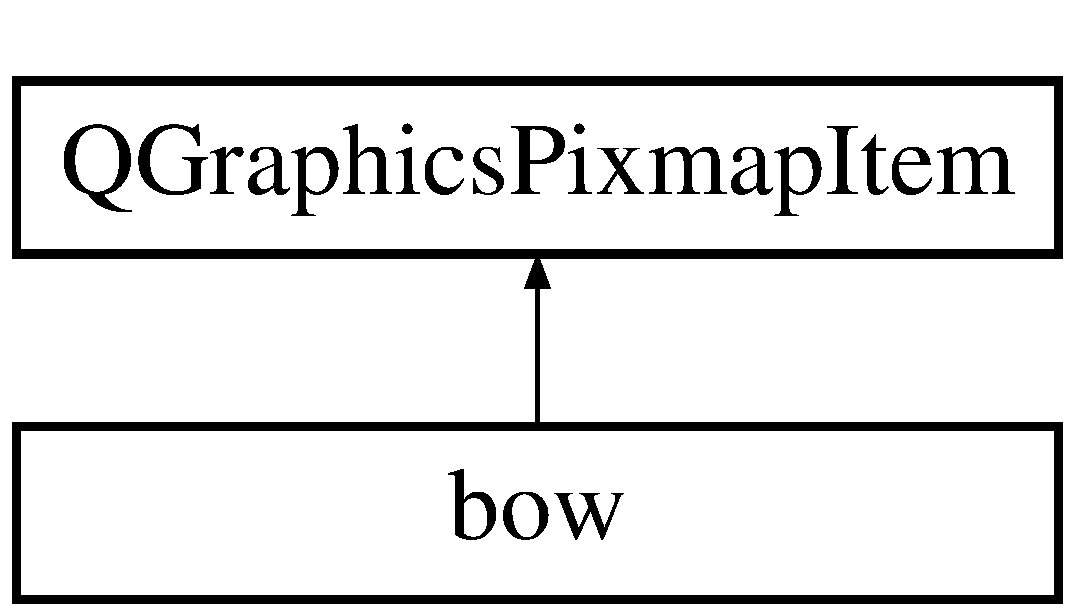
\includegraphics[height=2.000000cm]{classbow}
\end{center}
\end{figure}
\subsection*{Public Member Functions}
\begin{DoxyCompactItemize}
\item 
\mbox{\Hypertarget{classbow_a0f2eebc1d7b9c9d6522837c754c109ab}\label{classbow_a0f2eebc1d7b9c9d6522837c754c109ab}} 
\hyperlink{classbow_a0f2eebc1d7b9c9d6522837c754c109ab}{bow} ()
\begin{DoxyCompactList}\small\item\em Bow Constructor. \end{DoxyCompactList}\end{DoxyCompactItemize}
\subsection*{Public Attributes}
\begin{DoxyCompactItemize}
\item 
\mbox{\Hypertarget{classbow_afe253300dbd500d2a937acd76af8f2cb}\label{classbow_afe253300dbd500d2a937acd76af8f2cb}} 
qreal \hyperlink{classbow_afe253300dbd500d2a937acd76af8f2cb}{angle}
\begin{DoxyCompactList}\small\item\em Angle of the Bow. \end{DoxyCompactList}\end{DoxyCompactItemize}


\subsection{Detailed Description}
The Class to create Bow object. 

The documentation for this class was generated from the following files\+:\begin{DoxyCompactItemize}
\item 
bow.\+h\item 
bow.\+cpp\end{DoxyCompactItemize}

\hypertarget{classclient}{}\section{client Class Reference}
\label{classclient}\index{client@{client}}


Classs to Create Client.  




{\ttfamily \#include $<$client.\+h$>$}

Inheritance diagram for client\+:\begin{figure}[H]
\begin{center}
\leavevmode
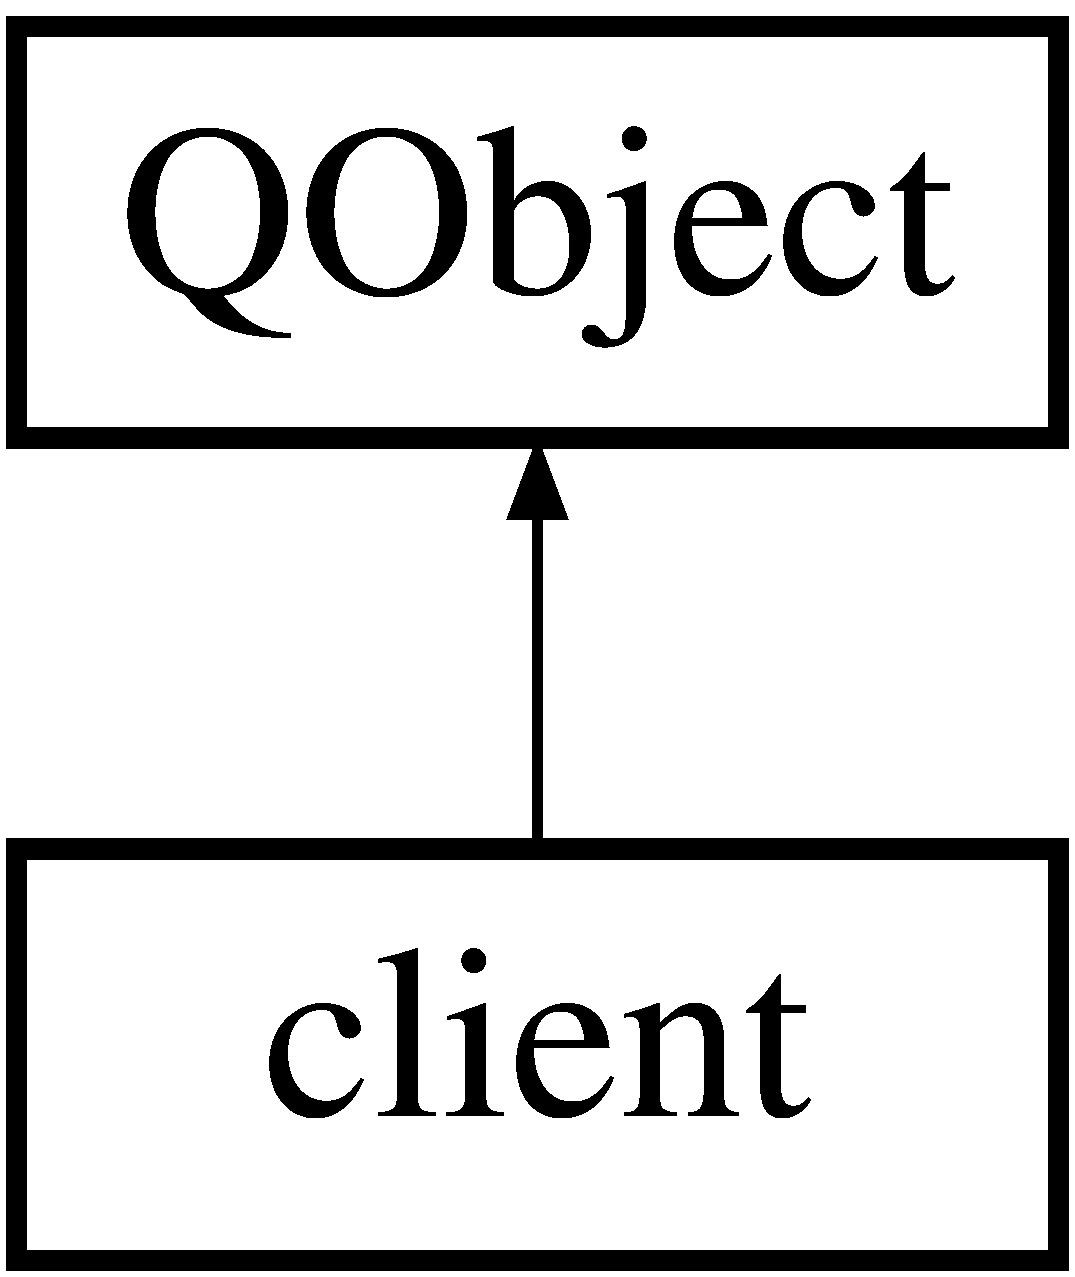
\includegraphics[height=2.000000cm]{classclient}
\end{center}
\end{figure}
\subsection*{Public Member Functions}
\begin{DoxyCompactItemize}
\item 
\hyperlink{classclient_a9ea8d82dfe1a28c0e44d37a61eedef8d}{client} (\hyperlink{classgamestate}{gamestate} $\ast$state\+\_\+param)
\begin{DoxyCompactList}\small\item\em Client Constructor. \end{DoxyCompactList}\item 
void \hyperlink{classclient_a573ec47d9b5e3829ea9eab522dd17394}{est\+Server\+Connection} (Q\+Url url\+\_\+param)
\begin{DoxyCompactList}\small\item\em TO Establish Connection between Server and C\+Lient. \end{DoxyCompactList}\end{DoxyCompactItemize}
\subsection*{Public Attributes}
\begin{DoxyCompactItemize}
\item 
\mbox{\Hypertarget{classclient_a7e0f2990d3dcaaf5347ee0ed4a863e86}\label{classclient_a7e0f2990d3dcaaf5347ee0ed4a863e86}} 
\hyperlink{classgamestate}{gamestate} $\ast$ \hyperlink{classclient_a7e0f2990d3dcaaf5347ee0ed4a863e86}{state}
\begin{DoxyCompactList}\small\item\em Reference to the state of the game. \end{DoxyCompactList}\end{DoxyCompactItemize}


\subsection{Detailed Description}
Classs to Create Client. 

\subsection{Constructor \& Destructor Documentation}
\mbox{\Hypertarget{classclient_a9ea8d82dfe1a28c0e44d37a61eedef8d}\label{classclient_a9ea8d82dfe1a28c0e44d37a61eedef8d}} 
\index{client@{client}!client@{client}}
\index{client@{client}!client@{client}}
\subsubsection{\texorpdfstring{client()}{client()}}
{\footnotesize\ttfamily client\+::client (\begin{DoxyParamCaption}\item[{\hyperlink{classgamestate}{gamestate} $\ast$}]{state\+\_\+param }\end{DoxyParamCaption})}



Client Constructor. 


\begin{DoxyParams}{Parameters}
{\em state\+\_\+param} & State of the Game \\
\hline
\end{DoxyParams}


\subsection{Member Function Documentation}
\mbox{\Hypertarget{classclient_a573ec47d9b5e3829ea9eab522dd17394}\label{classclient_a573ec47d9b5e3829ea9eab522dd17394}} 
\index{client@{client}!est\+Server\+Connection@{est\+Server\+Connection}}
\index{est\+Server\+Connection@{est\+Server\+Connection}!client@{client}}
\subsubsection{\texorpdfstring{est\+Server\+Connection()}{estServerConnection()}}
{\footnotesize\ttfamily void client\+::est\+Server\+Connection (\begin{DoxyParamCaption}\item[{Q\+Url}]{url\+\_\+param }\end{DoxyParamCaption})}



TO Establish Connection between Server and C\+Lient. 


\begin{DoxyParams}{Parameters}
{\em url\+\_\+param} & Server\textquotesingle{}s U\+RL \\
\hline
\end{DoxyParams}


The documentation for this class was generated from the following files\+:\begin{DoxyCompactItemize}
\item 
client.\+h\item 
client.\+cpp\end{DoxyCompactItemize}

\hypertarget{classgamestate}{}\section{gamestate Class Reference}
\label{classgamestate}\index{gamestate@{gamestate}}


Class to store the State of the Game.  




{\ttfamily \#include $<$gamestate.\+h$>$}

\subsection*{Public Member Functions}
\begin{DoxyCompactItemize}
\item 
\mbox{\Hypertarget{classgamestate_ab58660ea8cba18f34d30afdf9afeee3a}\label{classgamestate_ab58660ea8cba18f34d30afdf9afeee3a}} 
\hyperlink{classgamestate_ab58660ea8cba18f34d30afdf9afeee3a}{gamestate} (Q\+Graphics\+Scene $\ast$scene)
\begin{DoxyCompactList}\small\item\em Game\+State Constructor. \end{DoxyCompactList}\item 
\mbox{\Hypertarget{classgamestate_a2c5d0f47e823da319e366b4c3674520e}\label{classgamestate_a2c5d0f47e823da319e366b4c3674520e}} 
Q\+Json\+Object \hyperlink{classgamestate_a2c5d0f47e823da319e366b4c3674520e}{get\+Json\+Object} ()
\begin{DoxyCompactList}\small\item\em To get the Json Object of the Game\+State. \end{DoxyCompactList}\end{DoxyCompactItemize}
\subsection*{Public Attributes}
\begin{DoxyCompactItemize}
\item 
\mbox{\Hypertarget{classgamestate_acb59a99cf8d8582c1f9f81a83f2f5f73}\label{classgamestate_acb59a99cf8d8582c1f9f81a83f2f5f73}} 
int \hyperlink{classgamestate_acb59a99cf8d8582c1f9f81a83f2f5f73}{id}
\begin{DoxyCompactList}\small\item\em id = 0 in Server and id = 1 in Client \end{DoxyCompactList}\item 
\mbox{\Hypertarget{classgamestate_a54c8ade27ab0bc446c9c178d15a2e9c5}\label{classgamestate_a54c8ade27ab0bc446c9c178d15a2e9c5}} 
Q\+Graphics\+Scene $\ast$ \hyperlink{classgamestate_a54c8ade27ab0bc446c9c178d15a2e9c5}{state\+Scene}
\begin{DoxyCompactList}\small\item\em Reference to the scene in the game. \end{DoxyCompactList}\item 
\mbox{\Hypertarget{classgamestate_a5c3589f6ddece131a18e3c725c0deace}\label{classgamestate_a5c3589f6ddece131a18e3c725c0deace}} 
Q\+PointF \hyperlink{classgamestate_a5c3589f6ddece131a18e3c725c0deace}{Player1\+Position}
\begin{DoxyCompactList}\small\item\em Stores the position of Player 1. \end{DoxyCompactList}\item 
\mbox{\Hypertarget{classgamestate_a27d4875191db36c69f2c1e0604ebf36f}\label{classgamestate_a27d4875191db36c69f2c1e0604ebf36f}} 
Q\+PointF \hyperlink{classgamestate_a27d4875191db36c69f2c1e0604ebf36f}{Player2\+Position}
\begin{DoxyCompactList}\small\item\em Stores the position of Player 2. \end{DoxyCompactList}\item 
\mbox{\Hypertarget{classgamestate_a5767b07aaa2c0bd46ff55795be98b440}\label{classgamestate_a5767b07aaa2c0bd46ff55795be98b440}} 
Q\+PointF \hyperlink{classgamestate_a5767b07aaa2c0bd46ff55795be98b440}{Target\+Position}
\begin{DoxyCompactList}\small\item\em Stores the position of the Target. \end{DoxyCompactList}\item 
\mbox{\Hypertarget{classgamestate_a4883320071dbaf4e4bb455035b7847a2}\label{classgamestate_a4883320071dbaf4e4bb455035b7847a2}} 
bool \hyperlink{classgamestate_a4883320071dbaf4e4bb455035b7847a2}{is\+Arrow1}
\begin{DoxyCompactList}\small\item\em Tells if the arrow of player 1 is in the scene. \end{DoxyCompactList}\item 
\mbox{\Hypertarget{classgamestate_a216b721f59c27708fbd0bf1e46a11642}\label{classgamestate_a216b721f59c27708fbd0bf1e46a11642}} 
bool \hyperlink{classgamestate_a216b721f59c27708fbd0bf1e46a11642}{is\+Arrow2}
\begin{DoxyCompactList}\small\item\em Tells if the arrow of player 2 is in the scene. \end{DoxyCompactList}\item 
\mbox{\Hypertarget{classgamestate_a25fbcaf81c3ce110b327fe86528de87a}\label{classgamestate_a25fbcaf81c3ce110b327fe86528de87a}} 
Q\+PointF \hyperlink{classgamestate_a25fbcaf81c3ce110b327fe86528de87a}{Arrow1\+Position}
\begin{DoxyCompactList}\small\item\em Stores the position of Arrow 1. \end{DoxyCompactList}\item 
\mbox{\Hypertarget{classgamestate_af99cef79dd656dabaa8bf633a5df48a3}\label{classgamestate_af99cef79dd656dabaa8bf633a5df48a3}} 
qreal \hyperlink{classgamestate_af99cef79dd656dabaa8bf633a5df48a3}{Arrow1\+Angle}
\begin{DoxyCompactList}\small\item\em Stores the angle of Arrow 1. \end{DoxyCompactList}\item 
\mbox{\Hypertarget{classgamestate_aeceed910e563d8a01b4eb690802f09a3}\label{classgamestate_aeceed910e563d8a01b4eb690802f09a3}} 
qreal \hyperlink{classgamestate_aeceed910e563d8a01b4eb690802f09a3}{Arrow2\+Angle}
\begin{DoxyCompactList}\small\item\em Stores the angle of Arrow 2. \end{DoxyCompactList}\item 
\mbox{\Hypertarget{classgamestate_a7dd00d203a53870b8fb0ddc1958ca5e6}\label{classgamestate_a7dd00d203a53870b8fb0ddc1958ca5e6}} 
Q\+PointF \hyperlink{classgamestate_a7dd00d203a53870b8fb0ddc1958ca5e6}{Arrow2\+Position}
\begin{DoxyCompactList}\small\item\em Stores the position of Arrow 2. \end{DoxyCompactList}\item 
\mbox{\Hypertarget{classgamestate_ad4ce2f0afef6a295020a0939a9ab2679}\label{classgamestate_ad4ce2f0afef6a295020a0939a9ab2679}} 
qreal \hyperlink{classgamestate_ad4ce2f0afef6a295020a0939a9ab2679}{Bow1\+Angle}
\begin{DoxyCompactList}\small\item\em Stores the angle of Bow 1. \end{DoxyCompactList}\item 
\mbox{\Hypertarget{classgamestate_a6a224fa2eba20bda148712d3a9908e47}\label{classgamestate_a6a224fa2eba20bda148712d3a9908e47}} 
qreal \hyperlink{classgamestate_a6a224fa2eba20bda148712d3a9908e47}{Bow2\+Angle}
\begin{DoxyCompactList}\small\item\em Stores the angle of Bow 2. \end{DoxyCompactList}\item 
\mbox{\Hypertarget{classgamestate_aa278aeddb0187a556914fb50dbca5449}\label{classgamestate_aa278aeddb0187a556914fb50dbca5449}} 
int \hyperlink{classgamestate_aa278aeddb0187a556914fb50dbca5449}{hit}
\begin{DoxyCompactList}\small\item\em Tells if the arrow of client had hit the target. \end{DoxyCompactList}\item 
\mbox{\Hypertarget{classgamestate_a0101bc9654cb25898514da6e5b614dc2}\label{classgamestate_a0101bc9654cb25898514da6e5b614dc2}} 
int \hyperlink{classgamestate_a0101bc9654cb25898514da6e5b614dc2}{points1}
\begin{DoxyCompactList}\small\item\em Stores the score of Player 1. \end{DoxyCompactList}\item 
\mbox{\Hypertarget{classgamestate_a9fc1884d54b5d42554a784749cad7025}\label{classgamestate_a9fc1884d54b5d42554a784749cad7025}} 
int \hyperlink{classgamestate_a9fc1884d54b5d42554a784749cad7025}{points2}
\begin{DoxyCompactList}\small\item\em Stores the score of Player 2. \end{DoxyCompactList}\end{DoxyCompactItemize}


\subsection{Detailed Description}
Class to store the State of the Game. 

The documentation for this class was generated from the following files\+:\begin{DoxyCompactItemize}
\item 
gamestate.\+h\item 
gamestate.\+cpp\end{DoxyCompactItemize}

\hypertarget{classmyplayer1}{}\section{myplayer1 Class Reference}
\label{classmyplayer1}\index{myplayer1@{myplayer1}}


Class to create Player Object.  




{\ttfamily \#include $<$myplayer1.\+h$>$}

Inheritance diagram for myplayer1\+:\begin{figure}[H]
\begin{center}
\leavevmode
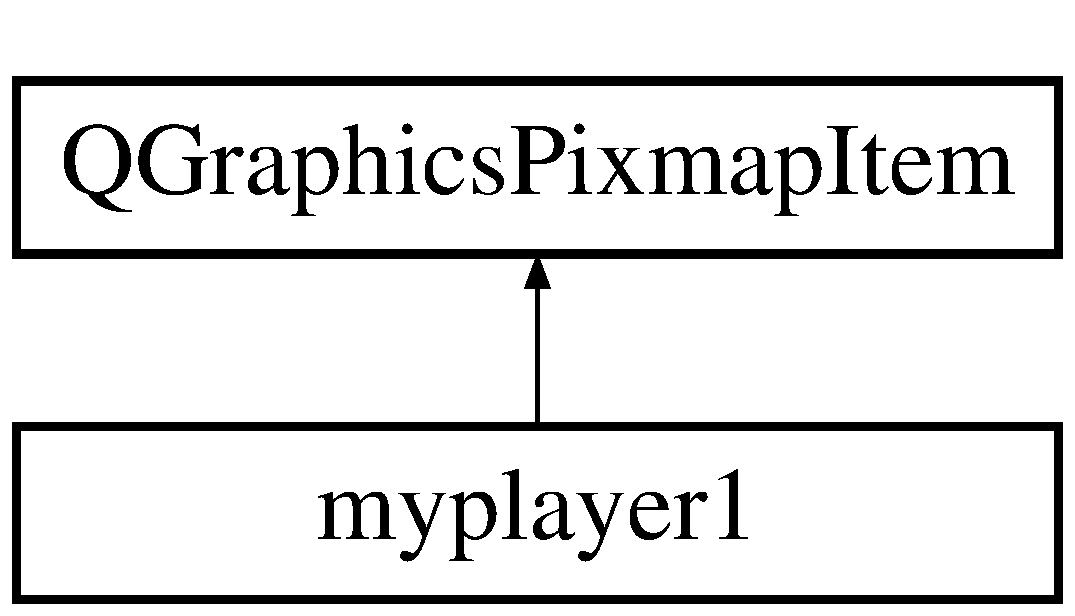
\includegraphics[height=2.000000cm]{classmyplayer1}
\end{center}
\end{figure}
\subsection*{Public Member Functions}
\begin{DoxyCompactItemize}
\item 
\hyperlink{classmyplayer1_a432fa3b50d94486945e6632035fdb79c}{myplayer1} (\hyperlink{classgamestate}{gamestate} $\ast$state\+\_\+param, \hyperlink{classtarget}{target} $\ast$t\+\_\+param)
\begin{DoxyCompactList}\small\item\em Player Constructor to create player 1. \end{DoxyCompactList}\item 
\mbox{\Hypertarget{classmyplayer1_a0313d001b5c663fc875c440cbafaefe0}\label{classmyplayer1_a0313d001b5c663fc875c440cbafaefe0}} 
\hyperlink{classmyplayer1_a0313d001b5c663fc875c440cbafaefe0}{myplayer1} (int i, \hyperlink{classgamestate}{gamestate} $\ast$state\+\_\+param)
\begin{DoxyCompactList}\small\item\em Player Constructor to create player 2. \end{DoxyCompactList}\item 
\mbox{\Hypertarget{classmyplayer1_a12d8f91b8542cf36072da7ff7b9ad524}\label{classmyplayer1_a12d8f91b8542cf36072da7ff7b9ad524}} 
void \hyperlink{classmyplayer1_a12d8f91b8542cf36072da7ff7b9ad524}{key\+Press\+Event} (Q\+Key\+Event $\ast$event)
\begin{DoxyCompactList}\small\item\em To process when a key is pressed by the user. \end{DoxyCompactList}\item 
\mbox{\Hypertarget{classmyplayer1_a94d95265e865928930664ef94fdc640b}\label{classmyplayer1_a94d95265e865928930664ef94fdc640b}} 
void \hyperlink{classmyplayer1_a94d95265e865928930664ef94fdc640b}{set\+Client\+Local} (Q\+Web\+Socket $\ast$client\+\_\+param)
\begin{DoxyCompactList}\small\item\em Function to set the reference to the Client Socket in the game. \end{DoxyCompactList}\end{DoxyCompactItemize}
\subsection*{Public Attributes}
\begin{DoxyCompactItemize}
\item 
\mbox{\Hypertarget{classmyplayer1_ab0cafd2fa2aa3e035a614971cc6a362e}\label{classmyplayer1_ab0cafd2fa2aa3e035a614971cc6a362e}} 
\hyperlink{classbow}{bow} $\ast$ \hyperlink{classmyplayer1_ab0cafd2fa2aa3e035a614971cc6a362e}{bow1}
\begin{DoxyCompactList}\small\item\em Reference to the bow of the player. \end{DoxyCompactList}\item 
\mbox{\Hypertarget{classmyplayer1_a507ebf8c50ae21fe3c8b0a89dd27713a}\label{classmyplayer1_a507ebf8c50ae21fe3c8b0a89dd27713a}} 
\hyperlink{classgamestate}{gamestate} $\ast$ \hyperlink{classmyplayer1_a507ebf8c50ae21fe3c8b0a89dd27713a}{state}
\begin{DoxyCompactList}\small\item\em Reference to the state of the game. \end{DoxyCompactList}\item 
\mbox{\Hypertarget{classmyplayer1_aedcf8f8e414e01203289b4ba6355bf01}\label{classmyplayer1_aedcf8f8e414e01203289b4ba6355bf01}} 
\hyperlink{classtarget}{target} $\ast$ \hyperlink{classmyplayer1_aedcf8f8e414e01203289b4ba6355bf01}{t}
\begin{DoxyCompactList}\small\item\em Reference to the target in the game. \end{DoxyCompactList}\item 
\mbox{\Hypertarget{classmyplayer1_ae95fc3dcaf03caa5fdfb1deb5ecc5c5c}\label{classmyplayer1_ae95fc3dcaf03caa5fdfb1deb5ecc5c5c}} 
\hyperlink{classarrow}{arrow} $\ast$ \hyperlink{classmyplayer1_ae95fc3dcaf03caa5fdfb1deb5ecc5c5c}{player2\+Arrow}
\begin{DoxyCompactList}\small\item\em Reference to the arrow of player 2. \end{DoxyCompactList}\item 
\mbox{\Hypertarget{classmyplayer1_a58c818ae137860bfdd64197e37f25371}\label{classmyplayer1_a58c818ae137860bfdd64197e37f25371}} 
Q\+Web\+Socket $\ast$ \hyperlink{classmyplayer1_a58c818ae137860bfdd64197e37f25371}{client\+\_\+local}
\begin{DoxyCompactList}\small\item\em Reference to the Client Socket in the game. \end{DoxyCompactList}\end{DoxyCompactItemize}


\subsection{Detailed Description}
Class to create Player Object. 

\subsection{Constructor \& Destructor Documentation}
\mbox{\Hypertarget{classmyplayer1_a432fa3b50d94486945e6632035fdb79c}\label{classmyplayer1_a432fa3b50d94486945e6632035fdb79c}} 
\index{myplayer1@{myplayer1}!myplayer1@{myplayer1}}
\index{myplayer1@{myplayer1}!myplayer1@{myplayer1}}
\subsubsection{\texorpdfstring{myplayer1()}{myplayer1()}}
{\footnotesize\ttfamily myplayer1\+::myplayer1 (\begin{DoxyParamCaption}\item[{\hyperlink{classgamestate}{gamestate} $\ast$}]{state\+\_\+param,  }\item[{\hyperlink{classtarget}{target} $\ast$}]{t\+\_\+param }\end{DoxyParamCaption})}



Player Constructor to create player 1. 


\begin{DoxyParams}{Parameters}
{\em state\+\_\+param} & State of the Game \\
\hline
{\em t\+\_\+param} & Target in the Game \\
\hline
\end{DoxyParams}


The documentation for this class was generated from the following files\+:\begin{DoxyCompactItemize}
\item 
myplayer1.\+h\item 
myplayer1.\+cpp\end{DoxyCompactItemize}

\hypertarget{classscore}{}\section{score Class Reference}
\label{classscore}\index{score@{score}}


Class to create Score Object.  




{\ttfamily \#include $<$score.\+h$>$}

Inheritance diagram for score\+:\begin{figure}[H]
\begin{center}
\leavevmode
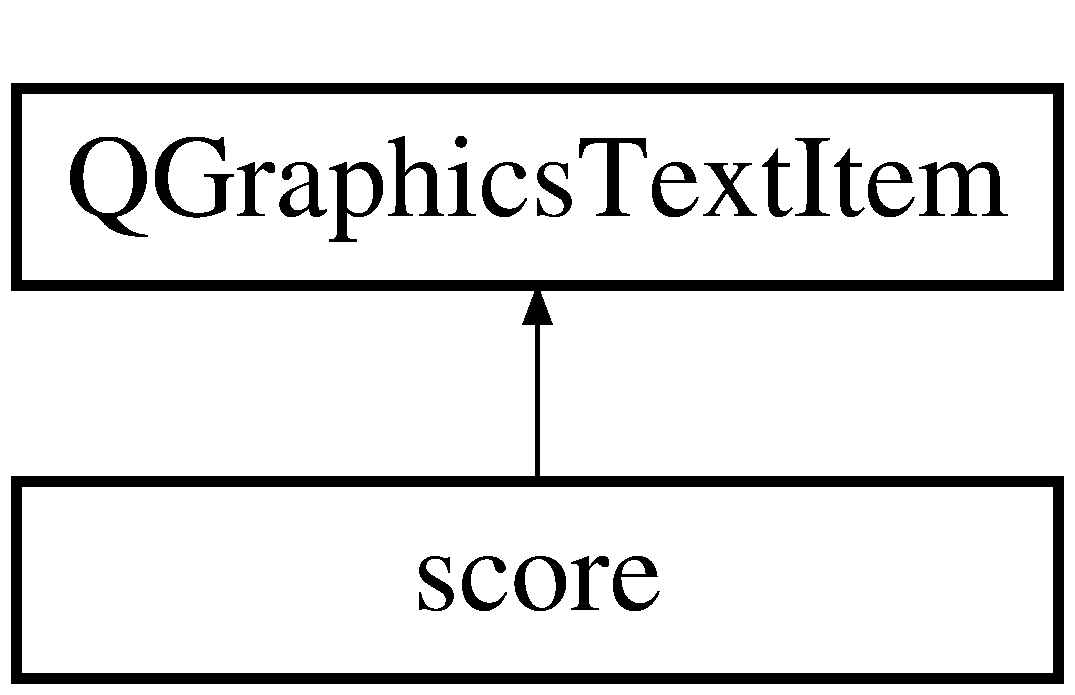
\includegraphics[height=2.000000cm]{classscore}
\end{center}
\end{figure}
\subsection*{Public Member Functions}
\begin{DoxyCompactItemize}
\item 
\mbox{\Hypertarget{classscore_aaf1ad193f5292e86d471d6bbd5d87cfb}\label{classscore_aaf1ad193f5292e86d471d6bbd5d87cfb}} 
\hyperlink{classscore_aaf1ad193f5292e86d471d6bbd5d87cfb}{score} (Q\+Graphics\+Item $\ast$parent=0)
\begin{DoxyCompactList}\small\item\em Score Constructor. \end{DoxyCompactList}\item 
\mbox{\Hypertarget{classscore_a0544bdc07cf845e67e978111b6166297}\label{classscore_a0544bdc07cf845e67e978111b6166297}} 
void \hyperlink{classscore_a0544bdc07cf845e67e978111b6166297}{increase} ()
\begin{DoxyCompactList}\small\item\em Increments the Score by 1. \end{DoxyCompactList}\item 
\mbox{\Hypertarget{classscore_a1556ae2741d225c184f5869ccf8082b8}\label{classscore_a1556ae2741d225c184f5869ccf8082b8}} 
int \hyperlink{classscore_a1556ae2741d225c184f5869ccf8082b8}{get\+Score} ()
\begin{DoxyCompactList}\small\item\em Returns the Score. \end{DoxyCompactList}\end{DoxyCompactItemize}


\subsection{Detailed Description}
Class to create Score Object. 

The documentation for this class was generated from the following files\+:\begin{DoxyCompactItemize}
\item 
score.\+h\item 
score.\+cpp\end{DoxyCompactItemize}

\hypertarget{classscoreboard}{}\section{scoreboard Class Reference}
\label{classscoreboard}\index{scoreboard@{scoreboard}}


Class to create Scoreboard Object.  




{\ttfamily \#include $<$scoreboard.\+h$>$}

Inheritance diagram for scoreboard\+:\begin{figure}[H]
\begin{center}
\leavevmode
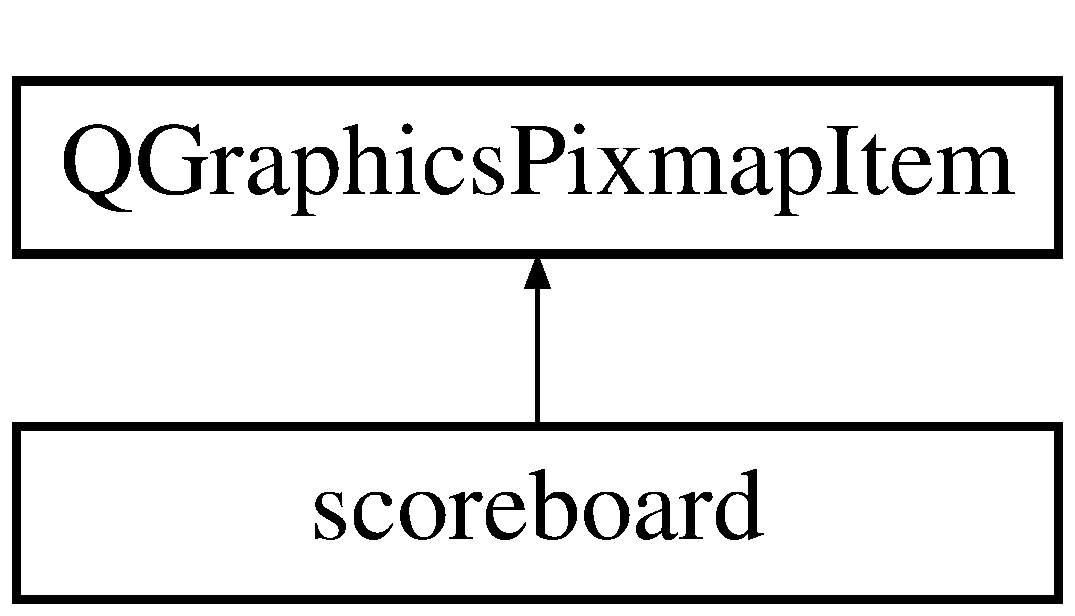
\includegraphics[height=2.000000cm]{classscoreboard}
\end{center}
\end{figure}
\subsection*{Public Member Functions}
\begin{DoxyCompactItemize}
\item 
\mbox{\Hypertarget{classscoreboard_a7e4efcdab636a3b259061e93d5f42b23}\label{classscoreboard_a7e4efcdab636a3b259061e93d5f42b23}} 
\hyperlink{classscoreboard_a7e4efcdab636a3b259061e93d5f42b23}{scoreboard} ()
\begin{DoxyCompactList}\small\item\em Scoreboard Constructor. \end{DoxyCompactList}\end{DoxyCompactItemize}


\subsection{Detailed Description}
Class to create Scoreboard Object. 

The documentation for this class was generated from the following files\+:\begin{DoxyCompactItemize}
\item 
scoreboard.\+h\item 
scoreboard.\+cpp\end{DoxyCompactItemize}

\hypertarget{classscreen_update}{}\section{screen\+Update Class Reference}
\label{classscreen_update}\index{screen\+Update@{screen\+Update}}


Class to create Screen Updator Object.  




{\ttfamily \#include $<$screenupdate.\+h$>$}

Inheritance diagram for screen\+Update\+:\begin{figure}[H]
\begin{center}
\leavevmode
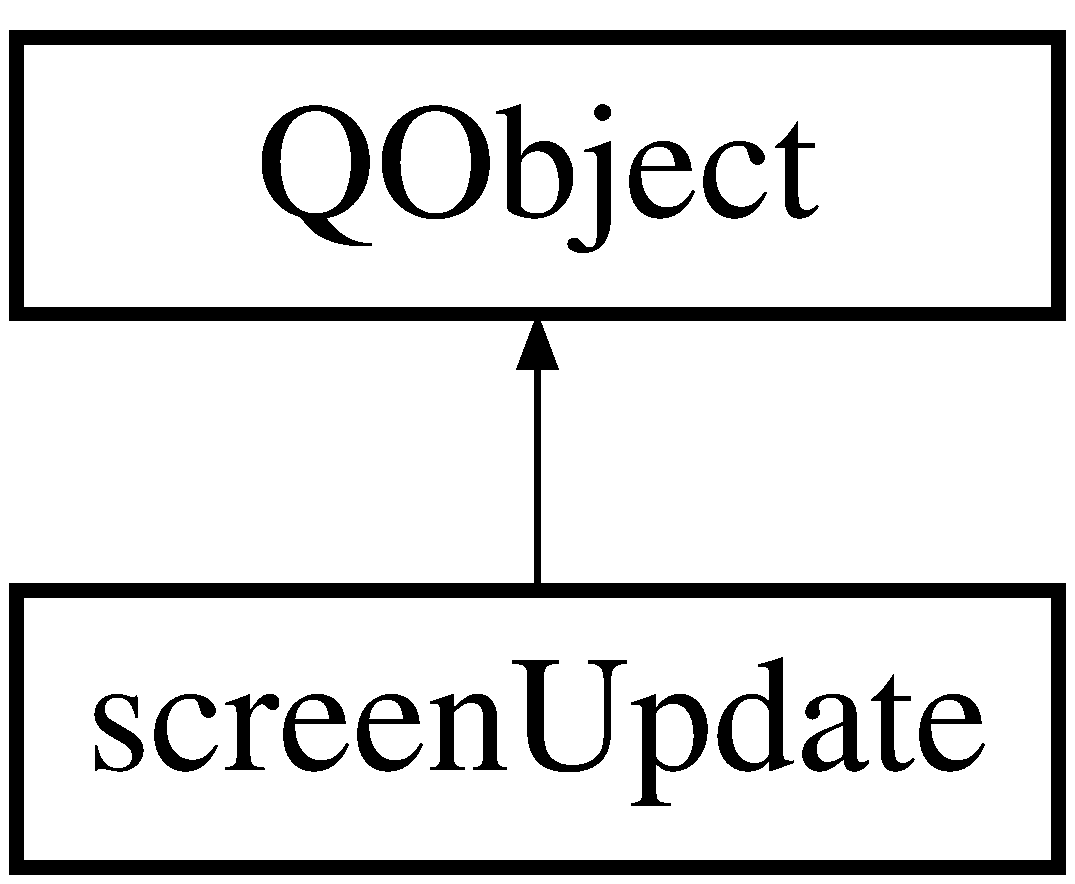
\includegraphics[height=2.000000cm]{classscreen_update}
\end{center}
\end{figure}
\subsection*{Public Member Functions}
\begin{DoxyCompactItemize}
\item 
\hyperlink{classscreen_update_ad92b56fb1e5fde3508070357acb89dfd}{screen\+Update} (Q\+Graphics\+Scene $\ast$scene\+\_\+param, \hyperlink{classgamestate}{gamestate} $\ast$state\+\_\+param, \hyperlink{classmyplayer1}{myplayer1} $\ast$p2\+\_\+param, int i, \hyperlink{classtarget}{target} $\ast$t\+\_\+param)
\begin{DoxyCompactList}\small\item\em screenupdate Constructor \end{DoxyCompactList}\item 
\mbox{\Hypertarget{classscreen_update_a23e41b958b924804dbe4986619c091d0}\label{classscreen_update_a23e41b958b924804dbe4986619c091d0}} 
void \hyperlink{classscreen_update_a23e41b958b924804dbe4986619c091d0}{start\+Update} ()
\begin{DoxyCompactList}\small\item\em Calls the update() function using Q\+Timer. \end{DoxyCompactList}\end{DoxyCompactItemize}
\subsection*{Public Attributes}
\begin{DoxyCompactItemize}
\item 
\mbox{\Hypertarget{classscreen_update_a3ed9e1106e743e1d7916c6107237a6c6}\label{classscreen_update_a3ed9e1106e743e1d7916c6107237a6c6}} 
Q\+Graphics\+Scene $\ast$ \hyperlink{classscreen_update_a3ed9e1106e743e1d7916c6107237a6c6}{scene\+\_\+local}
\begin{DoxyCompactList}\small\item\em Reference to the scene of the game. \end{DoxyCompactList}\item 
\mbox{\Hypertarget{classscreen_update_a1022348c9f7f684ca3c8dc6bcb53c4b2}\label{classscreen_update_a1022348c9f7f684ca3c8dc6bcb53c4b2}} 
int \hyperlink{classscreen_update_a1022348c9f7f684ca3c8dc6bcb53c4b2}{id}
\begin{DoxyCompactList}\small\item\em Tells if Server or Client. \end{DoxyCompactList}\item 
\mbox{\Hypertarget{classscreen_update_a8177d584c17e9018da226571c6789724}\label{classscreen_update_a8177d584c17e9018da226571c6789724}} 
\hyperlink{classmyplayer1}{myplayer1} $\ast$ \hyperlink{classscreen_update_a8177d584c17e9018da226571c6789724}{p1}
\begin{DoxyCompactList}\small\item\em Reference to player 1. \end{DoxyCompactList}\item 
\mbox{\Hypertarget{classscreen_update_a7b1fa00ae6daac23742776f647df7d52}\label{classscreen_update_a7b1fa00ae6daac23742776f647df7d52}} 
\hyperlink{classmyplayer1}{myplayer1} $\ast$ \hyperlink{classscreen_update_a7b1fa00ae6daac23742776f647df7d52}{p2}
\begin{DoxyCompactList}\small\item\em Reference to player 2. \end{DoxyCompactList}\item 
\mbox{\Hypertarget{classscreen_update_a60461a2c1374a3de8c3690b4a9407515}\label{classscreen_update_a60461a2c1374a3de8c3690b4a9407515}} 
\hyperlink{classtarget}{target} $\ast$ \hyperlink{classscreen_update_a60461a2c1374a3de8c3690b4a9407515}{t}
\begin{DoxyCompactList}\small\item\em Reference to Target. \end{DoxyCompactList}\item 
\mbox{\Hypertarget{classscreen_update_ac93039dd4a91aa32acbcc656695a3185}\label{classscreen_update_ac93039dd4a91aa32acbcc656695a3185}} 
\hyperlink{classgamestate}{gamestate} $\ast$ \hyperlink{classscreen_update_ac93039dd4a91aa32acbcc656695a3185}{state}
\begin{DoxyCompactList}\small\item\em Reference to the state of the game. \end{DoxyCompactList}\end{DoxyCompactItemize}


\subsection{Detailed Description}
Class to create Screen Updator Object. 

\subsection{Constructor \& Destructor Documentation}
\mbox{\Hypertarget{classscreen_update_ad92b56fb1e5fde3508070357acb89dfd}\label{classscreen_update_ad92b56fb1e5fde3508070357acb89dfd}} 
\index{screen\+Update@{screen\+Update}!screen\+Update@{screen\+Update}}
\index{screen\+Update@{screen\+Update}!screen\+Update@{screen\+Update}}
\subsubsection{\texorpdfstring{screen\+Update()}{screenUpdate()}}
{\footnotesize\ttfamily screen\+Update\+::screen\+Update (\begin{DoxyParamCaption}\item[{Q\+Graphics\+Scene $\ast$}]{scene\+\_\+param,  }\item[{\hyperlink{classgamestate}{gamestate} $\ast$}]{state\+\_\+param,  }\item[{\hyperlink{classmyplayer1}{myplayer1} $\ast$}]{p2\+\_\+param,  }\item[{int}]{i,  }\item[{\hyperlink{classtarget}{target} $\ast$}]{t\+\_\+param }\end{DoxyParamCaption})}



screenupdate Constructor 


\begin{DoxyParams}{Parameters}
{\em scene\+\_\+param} & Scene of the Game \\
\hline
{\em state\+\_\+param} & State of the Game \\
\hline
{\em p2\+\_\+param} & Player 2 of the Game \\
\hline
{\em i} & Id(\+Server or Client) \\
\hline
{\em t\+\_\+param} & Target of the Game \\
\hline
\end{DoxyParams}


The documentation for this class was generated from the following files\+:\begin{DoxyCompactItemize}
\item 
screenupdate.\+h\item 
screenupdate.\+cpp\end{DoxyCompactItemize}

\hypertarget{classserver}{}\section{server Class Reference}
\label{classserver}\index{server@{server}}


Class to create Server.  




{\ttfamily \#include $<$server.\+h$>$}

Inheritance diagram for server\+:\begin{figure}[H]
\begin{center}
\leavevmode
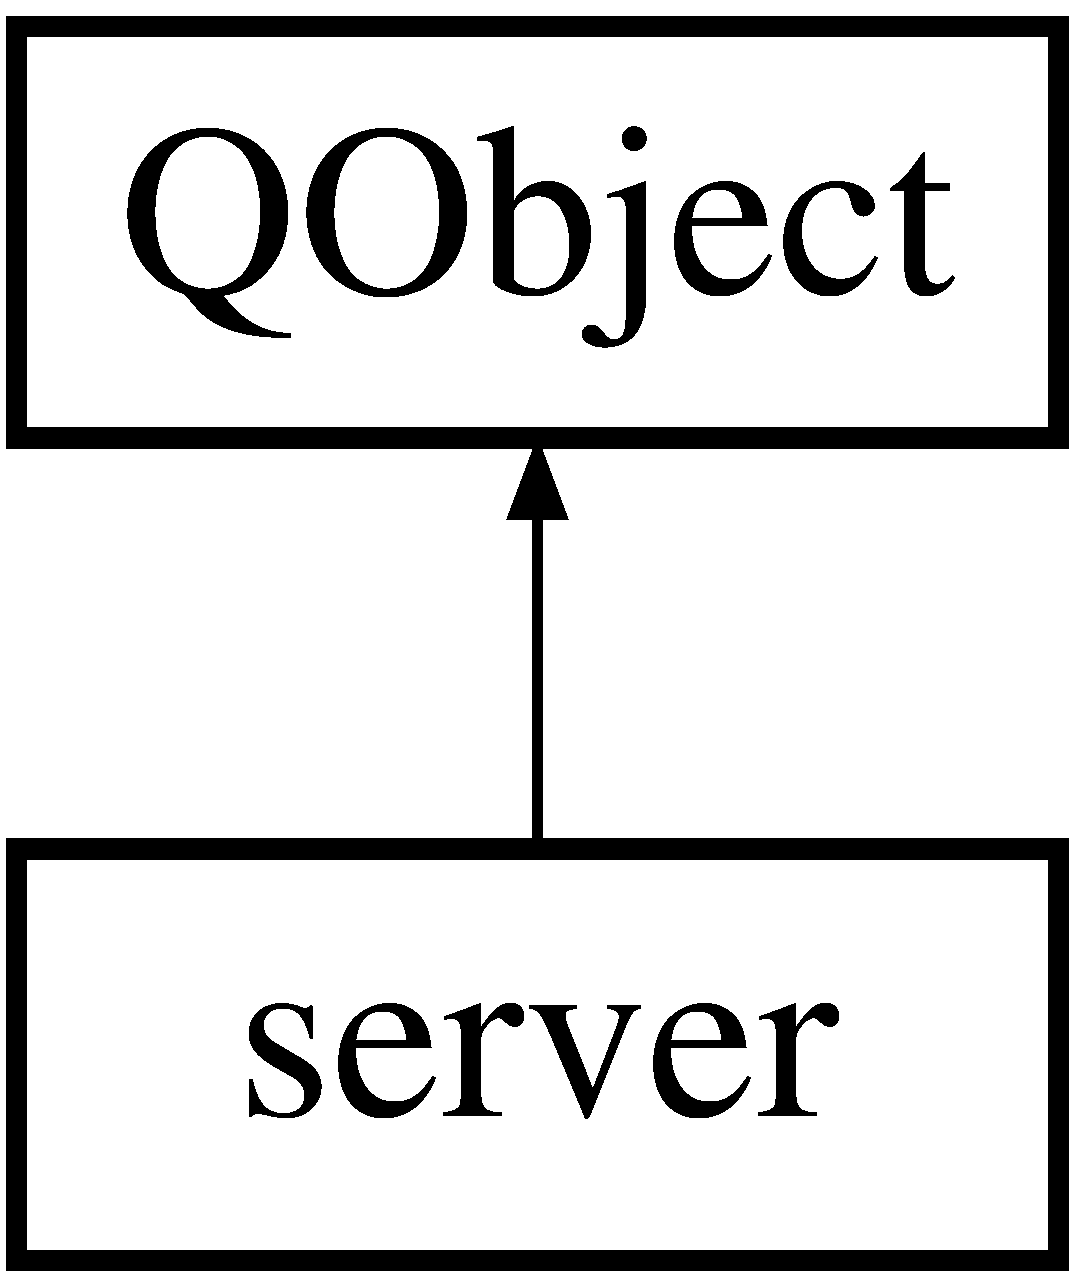
\includegraphics[height=2.000000cm]{classserver}
\end{center}
\end{figure}
\subsection*{Public Member Functions}
\begin{DoxyCompactItemize}
\item 
\hyperlink{classserver_a78f26aa936c3bf529e53d97d39842700}{server} (Q\+Graphics\+Scene $\ast$scene\+\_\+param, Q\+Graphics\+View $\ast$view\+\_\+param, quint16 port\+\_\+param, \hyperlink{classgamestate}{gamestate} $\ast$state\+\_\+param, \hyperlink{classtarget}{target} $\ast$t\+\_\+param)
\begin{DoxyCompactList}\small\item\em Server Constructor. \end{DoxyCompactList}\item 
\mbox{\Hypertarget{classserver_a4f2787ad7f4f65d5b010d0292a06c2d1}\label{classserver_a4f2787ad7f4f65d5b010d0292a06c2d1}} 
void \hyperlink{classserver_a4f2787ad7f4f65d5b010d0292a06c2d1}{start\+Server} ()
\begin{DoxyCompactList}\small\item\em Starts the server. \end{DoxyCompactList}\item 
\mbox{\Hypertarget{classserver_abae49f99fc3cc4a1490d66fb7ad7885e}\label{classserver_abae49f99fc3cc4a1490d66fb7ad7885e}} 
void \hyperlink{classserver_abae49f99fc3cc4a1490d66fb7ad7885e}{game\+Loop} ()
\begin{DoxyCompactList}\small\item\em Runs the Game loop. \end{DoxyCompactList}\end{DoxyCompactItemize}


\subsection{Detailed Description}
Class to create Server. 

\subsection{Constructor \& Destructor Documentation}
\mbox{\Hypertarget{classserver_a78f26aa936c3bf529e53d97d39842700}\label{classserver_a78f26aa936c3bf529e53d97d39842700}} 
\index{server@{server}!server@{server}}
\index{server@{server}!server@{server}}
\subsubsection{\texorpdfstring{server()}{server()}}
{\footnotesize\ttfamily server\+::server (\begin{DoxyParamCaption}\item[{Q\+Graphics\+Scene $\ast$}]{scene\+\_\+param,  }\item[{Q\+Graphics\+View $\ast$}]{view\+\_\+param,  }\item[{quint16}]{port\+\_\+param,  }\item[{\hyperlink{classgamestate}{gamestate} $\ast$}]{state\+\_\+param,  }\item[{\hyperlink{classtarget}{target} $\ast$}]{t\+\_\+param }\end{DoxyParamCaption})}



Server Constructor. 


\begin{DoxyParams}{Parameters}
{\em scene\+\_\+param} & Scene of the Game \\
\hline
{\em view\+\_\+param} & View of the Game \\
\hline
{\em port\+\_\+param} & Port for communication \\
\hline
{\em state\+\_\+param} & State of the Game \\
\hline
{\em t\+\_\+param} & Target \\
\hline
\end{DoxyParams}


The documentation for this class was generated from the following files\+:\begin{DoxyCompactItemize}
\item 
server.\+h\item 
server.\+cpp\end{DoxyCompactItemize}

\hypertarget{classtarget}{}\section{target Class Reference}
\label{classtarget}\index{target@{target}}


Class to create Target object.  




{\ttfamily \#include $<$target.\+h$>$}

Inheritance diagram for target\+:\begin{figure}[H]
\begin{center}
\leavevmode
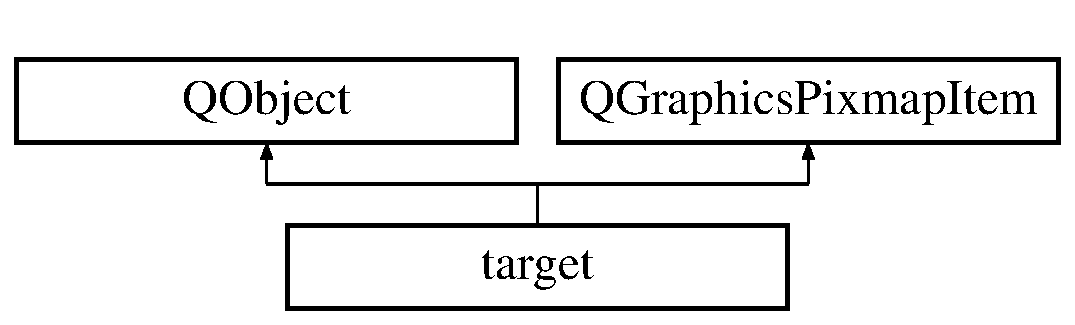
\includegraphics[height=2.000000cm]{classtarget}
\end{center}
\end{figure}
\subsection*{Public Slots}
\begin{DoxyCompactItemize}
\item 
\mbox{\Hypertarget{classtarget_a7ae097b44b076496d3a99ecd81bcc2e1}\label{classtarget_a7ae097b44b076496d3a99ecd81bcc2e1}} 
void \hyperlink{classtarget_a7ae097b44b076496d3a99ecd81bcc2e1}{move} ()
\begin{DoxyCompactList}\small\item\em moves the target \end{DoxyCompactList}\end{DoxyCompactItemize}
\subsection*{Public Member Functions}
\begin{DoxyCompactItemize}
\item 
\hyperlink{classtarget_a26ebddd755f8b29136be39b59b474b50}{target} (\hyperlink{classgamestate}{gamestate} $\ast$state\+\_\+param)
\begin{DoxyCompactList}\small\item\em Target Constructor fot Server. \end{DoxyCompactList}\item 
\hyperlink{classtarget_a091e064f965676275a1e86b09c3604b4}{target} (int i, \hyperlink{classgamestate}{gamestate} $\ast$state\+\_\+param)
\begin{DoxyCompactList}\small\item\em Target Constructor fot Client. \end{DoxyCompactList}\item 
\mbox{\Hypertarget{classtarget_a0d7ed50b67b1cacf5a7dc369b0b8c06d}\label{classtarget_a0d7ed50b67b1cacf5a7dc369b0b8c06d}} 
void \hyperlink{classtarget_a0d7ed50b67b1cacf5a7dc369b0b8c06d}{reset} ()
\begin{DoxyCompactList}\small\item\em Resets the position of the target. \end{DoxyCompactList}\end{DoxyCompactItemize}
\subsection*{Public Attributes}
\begin{DoxyCompactItemize}
\item 
\mbox{\Hypertarget{classtarget_a56a45205e30569263f53db4c5e91854c}\label{classtarget_a56a45205e30569263f53db4c5e91854c}} 
\hyperlink{classgamestate}{gamestate} $\ast$ \hyperlink{classtarget_a56a45205e30569263f53db4c5e91854c}{state}
\begin{DoxyCompactList}\small\item\em Reference to the state of the game. \end{DoxyCompactList}\item 
\mbox{\Hypertarget{classtarget_a2f109f42ea879dc7e6d186cfd5c605e4}\label{classtarget_a2f109f42ea879dc7e6d186cfd5c605e4}} 
int \hyperlink{classtarget_a2f109f42ea879dc7e6d186cfd5c605e4}{a}
\begin{DoxyCompactList}\small\item\em Stores the direction of movement of the target. \end{DoxyCompactList}\end{DoxyCompactItemize}


\subsection{Detailed Description}
Class to create Target object. 

\subsection{Constructor \& Destructor Documentation}
\mbox{\Hypertarget{classtarget_a26ebddd755f8b29136be39b59b474b50}\label{classtarget_a26ebddd755f8b29136be39b59b474b50}} 
\index{target@{target}!target@{target}}
\index{target@{target}!target@{target}}
\subsubsection{\texorpdfstring{target()}{target()}\hspace{0.1cm}{\footnotesize\ttfamily [1/2]}}
{\footnotesize\ttfamily target\+::target (\begin{DoxyParamCaption}\item[{\hyperlink{classgamestate}{gamestate} $\ast$}]{state\+\_\+param }\end{DoxyParamCaption})}



Target Constructor fot Server. 


\begin{DoxyParams}{Parameters}
{\em state\+\_\+param} & State of the game \\
\hline
\end{DoxyParams}
\mbox{\Hypertarget{classtarget_a091e064f965676275a1e86b09c3604b4}\label{classtarget_a091e064f965676275a1e86b09c3604b4}} 
\index{target@{target}!target@{target}}
\index{target@{target}!target@{target}}
\subsubsection{\texorpdfstring{target()}{target()}\hspace{0.1cm}{\footnotesize\ttfamily [2/2]}}
{\footnotesize\ttfamily target\+::target (\begin{DoxyParamCaption}\item[{int}]{i,  }\item[{\hyperlink{classgamestate}{gamestate} $\ast$}]{state\+\_\+param }\end{DoxyParamCaption})}



Target Constructor fot Client. 


\begin{DoxyParams}{Parameters}
{\em state\+\_\+param} & State of the Game \\
\hline
\end{DoxyParams}


The documentation for this class was generated from the following files\+:\begin{DoxyCompactItemize}
\item 
target.\+h\item 
target.\+cpp\end{DoxyCompactItemize}

%--- End generated contents ---

% Index
\backmatter
\newpage
\phantomsection
\clearemptydoublepage
\addcontentsline{toc}{chapter}{Index}
\printindex

\end{document}
